\begin{frame}{TLM (Transaction Level Modelling)}
\begin{block}{What is TLM?}
	\begin{itemize}
		\item Modelling styles and interoperability rules
  		\item Various levels of details of a design are modelled with one specification language
		\item Raise of abstraction level
	\end{itemize}
\end{block}
\begin{block}{Standard treat two different design issues}
	\begin{itemize}
		\item Communication
		\item Computation
	\end{itemize}	
\end{block}
\end{frame}
\begin{frame}{Virtual Platform Model}
\begin{block}{Purpose}
	\begin{itemize}
		\item TLM for architectural exploration and analysis
		\item Model for developing software applications with a reference model for hardware verification
		\item Available before final RTL exists
\end{itemize}
\end{block}
\begin{block}{Framework}
	\begin{itemize}
		\item Registers and functionality must be accurate
		\item No implementation details like pins or clock
		\item Approximate timing
		\item Fast enough to run software
	\end{itemize}
\end{block}
\end{frame}
\begin{frame}{TLM 2.0}
	\begin{itemize}
		\item OSCI (Open SystemC Initiative) TLM Standard \footnote{\url{https://www.accellera.org/images/downloads/standards/systemc/TLM_2_0_LRM.pdf}}
		\item Purpose Speed and Interoperability
		\item \textbf{Coding Styles:} Loosly Timed and Approximately Timed
	\end{itemize}
\begin{block}{Three Layers}
\begin{figure}
\label{fig:tlm2}
\centering
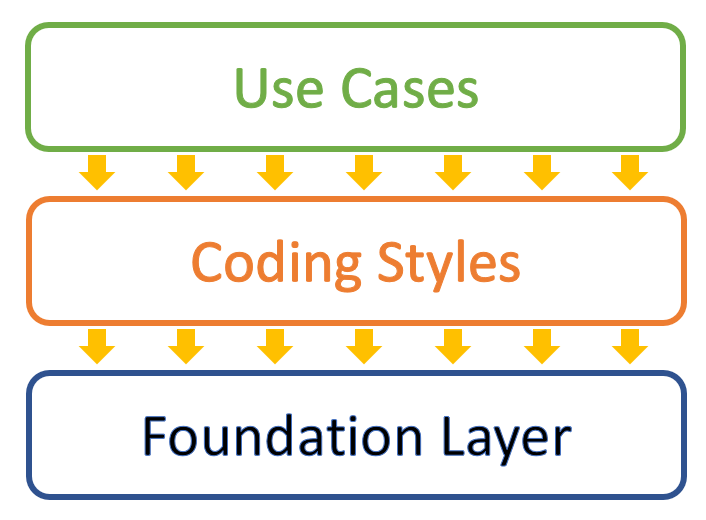
\includegraphics[width=0.5\textwidth]{pictures/Layers.PNG}
\end{figure}
\end{block}
\end{frame}
% \begin{frame}{Coding Styles}
% \begin{block}{Loosely Timed}
% 	\begin{itemize}
% 		\item Simulate as fast as possible
% 		\item Two main methods
% 		\begin{itemize}
% 			\item Temporal Decoupling
% 			\item Use direct memory interface (DMI)
% 		\end{itemize}
% 	\end{itemize}
% \end{block}
% \begin{block}{Approximately Timed}
% 	\begin{itemize}
% 		\item Just accurate enough for performance modelling
% 		\item Processes run in lock step with simulation time
% 	\end{itemize}
% \end{block}
% \end{frame}
\begin{frame}{Interoperability}
\begin{figure}
\label{fig:int}
\centering
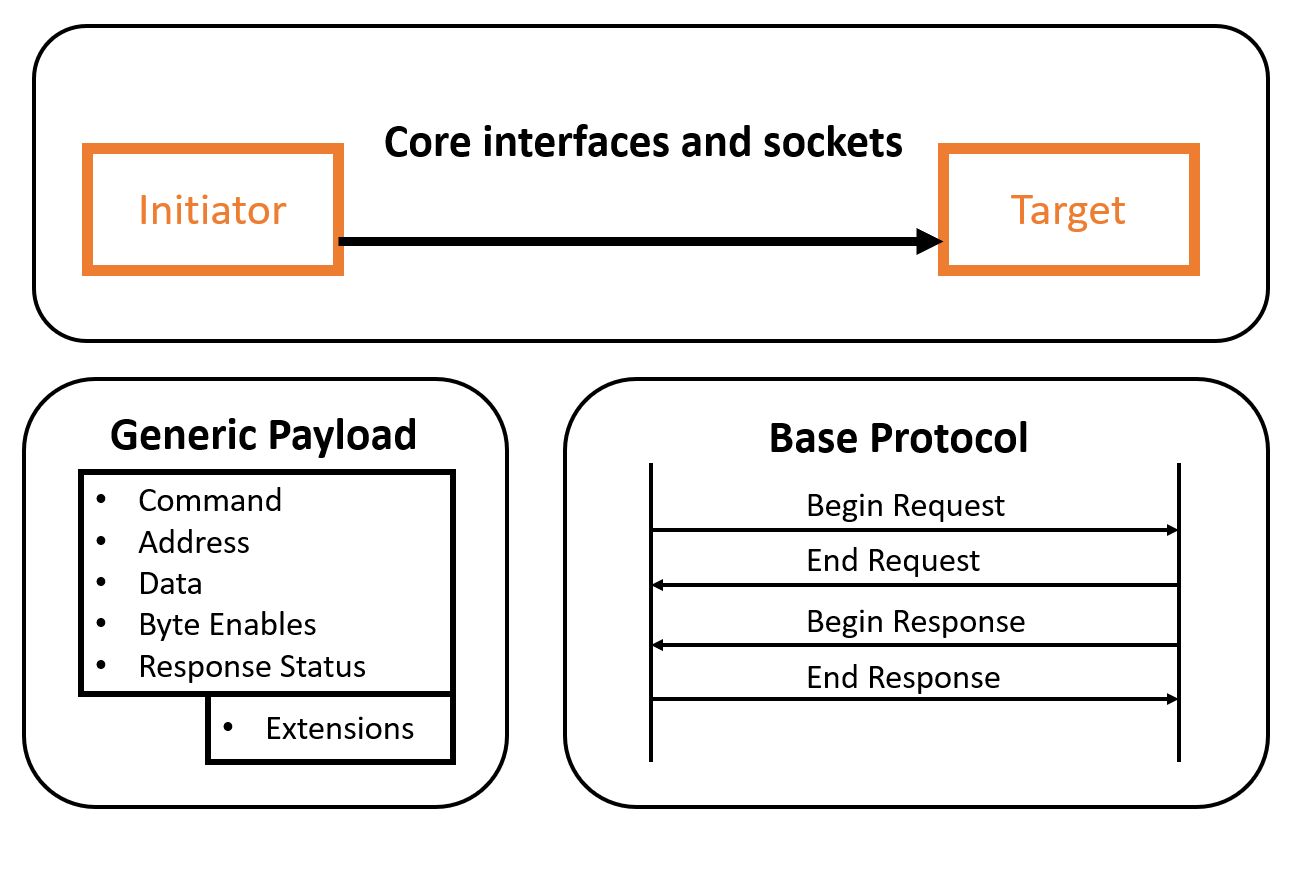
\includegraphics[width=0.9\textwidth]{pictures/Interoperability.PNG}
\end{figure}
\end{frame}
\begin{frame}{SoC Rocket Models Library}
Collection of different IP-Cores written in SystemC under the TLM IEEE Standard\footnote{T. Schuster et al. (2014). SoCRocket - A virtual platform for the European Space Agency's SoC development. 1-7.}
\begin{figure}
\label{fig:Lib}
\centering
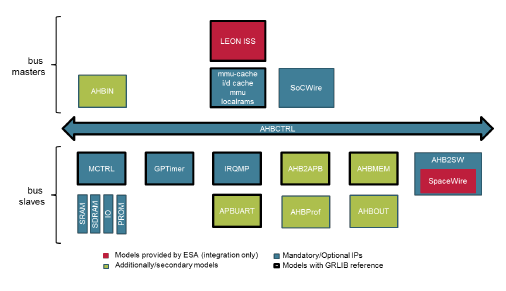
\includegraphics[width=1\textwidth]{pictures/ModelsLibrary.PNG}
\end{figure}
\end{frame}
